\documentclass[a4paper,12pt]{article}
\usepackage{amsmath}
\usepackage{amssymb}
\usepackage[polish]{babel}
\usepackage{polski}
\usepackage[utf8]{inputenc}
\usepackage{indentfirst}
\usepackage{geometry}
\usepackage{array}
\usepackage[pdftex]{color,graphicx}
\usepackage{subfigure}
\usepackage{afterpage}
\usepackage{setspace}
\usepackage{color}
\usepackage{wrapfig}
\usepackage{listings}
\usepackage{datetime}

\renewcommand{\onehalfspacing}{\setstretch{1.6}}

\geometry{tmargin=2.5cm,bmargin=2.5cm,lmargin=2.5cm,rmargin=2.5cm}
\setlength{\parindent}{1cm}
\setlength{\parskip}{0mm}

\newenvironment{lista}{
\begin{itemize}
  \setlength{\itemsep}{1pt}
  \setlength{\parskip}{0pt}
  \setlength{\parsep}{0pt}
}{\end{itemize}}

\newcommand{\linia}{\rule{\linewidth}{0.4mm}}

\definecolor{lbcolor}{rgb}{0.95,0.95,0.95}
\lstset{
    backgroundcolor=\color{lbcolor},
    tabsize=4,
  language=C++,
  captionpos=b,
  tabsize=3,
  frame=lines,
  numbers=left,
  numberstyle=\tiny,
  numbersep=5pt,
  breaklines=true,
  showstringspaces=false,
  basicstyle=\footnotesize,
  identifierstyle=\color{magenta},
  keywordstyle=\color[rgb]{0,0,1},
  commentstyle=\color{blue},
  stringstyle=\color{red}
  }

\begin{document}

\noindent
\begin{tabular}{|c|p{11cm}|c|} \hline 
Grupa 4 & Barbara Nowak, Piotr Tomaszewski & \ddmmyyyydate\formatdate{18}{01}{2017} \tabularnewline
\hline 
\end{tabular}


\section*{Zadanie 6 - Rozmycie Gaussa w CUDA}

Naszym zadaniem było zaimplementowanie programu, który rozmyje zadane zdjęcie (podobnie jak w zadaniach 4 i 5) ale stosując kartę graficzną i technologię CUDA.

Program uruchamiany jest z dwoma argumentami: pierwszy - to wybrany obrazek, a drugi - miejsce do zapisu zmodyfikowanego obrazka. Sprawdzamy czy program uruchamiany jest z wymaganą liczą argumentów wejściowych. 
Następnie deklarujemy maskę w postaci 2-wymiarowej tablicy liczb całkowitych oraz za pomocą funkcji imread(), wczytujemy wybrany plik do zmiennej zdjecie, a dzięki parametrowi CVxLOADxIMAGExCOLOR konwertujemy obrazek do wersji kolorowej. 
Kolejnym krokiem jest podział zadania na gridy(ilość bloków) oraz bloki(ilość wątków), który wyliczamy dzieląc odpowiednio kolumny i wiersze siatki zdjęcia przez ustalony rozmiar bloku równy 32. Następnie deklarujemy krotki dim3 do określenia wyliczonej wcześniej siatki oraz bloków.
\begin{lstlisting}
	int rozmiarBlok = 32;
	int rozmiarSiatkaSzer = zdj_we.cols/rozmiarBlok;
	int rozmiarSiatkaDlug = zdj_we.rows/rozmiarBlok;
	dim3 siatka(rozmiarSiatkaSzer, rozmiarSiatkaDlug);
	dim3 blok(rozmiarBlok, rozmiarBlok);
\end{lstlisting}

Tworzymy kopię wcześniej wczytanego zdjęcia do zmiennej zdjxwy.
Alokujemy pamięć na karcie graficznej dla wczytanego zdjęcia oraz dla jego kopii:
\begin{lstlisting}
	cudaMalloc(&zdj_gpu_we, zdj_we.rows*zdj_we.step*sizeof(unsigned char));
	cudaMalloc(&zdj_gpu_wy, zdj_we.rows*zdj_we.step*sizeof(unsigned char));
\end{lstlisting}

Kolejnym krokiem jest kopiowanie danych między kartą graficzną pamięcią RAM, gdzie obszar pamięci źródłowej należy do komputera (RAM), natomiast docelowy obszar pamięci należy 
do pamięci karty graficznej.
\begin{lstlisting}
	cudaMemcpy(zdj_gpu_we, zdj_we.ptr(), zdj_we.rows*zdj_we.step, cudaMemcpyHostToDevice);
\end{lstlisting}

Następnie rozpoczynamy pomiar czasu obliczeń pamiętając o użyciu cudaDeviceSynchronize(), która blokuje bieżący wątek aplikacji do czasu zakończenia wszystkich oczekiwanych obliczeń na karcie graficznej.
\begin{lstlisting}
	cudaEventRecord(czas_start, 0);
	rozmycie<<<siatka,blok>>>(zdj_we.channels(), sumaMaski(maska,0,0,0), zdj_gpu_we, zdj_gpu_wy, zdj_we.rows, zdj_we.step);
	cudaEventRecord(czas_stop, 0);
	cudaEventSynchronize(czas_stop);
	float czas = 0.0;
	cudaEventElapsedTime(&czas, czas_start, czas_stop);
	cudaDeviceSynchronize();
\end{lstlisting}

Ponownie kopiujemy dane między kartą graficzną a pamięcią RAM, jednak teraz obszar pamięci źródłowej należy do pamięci karty graficznej, natomiast docelowy obszar pamięci należy do komputera (RAM).
\begin{lstlisting}
	cudaMemcpy(zdj_wy.ptr(), zdj_gpu_wy, zdj_we.rows*zdj_we.step, cudaMemcpyDeviceToHost);
\end{lstlisting}

Na koniec pamiętamy o zwolnieniu pamięci wcześniej zaalokowanej na karcie graficznej, za pomocą funkcji cudaFree() oraz zapisujemy zmodyfikowany obrazek w miejsce zadane jako drugi argument.

\begin{wrapfigure}{r}{0.5\textwidth}
	\vspace{-40pt}
	\begin{center}
		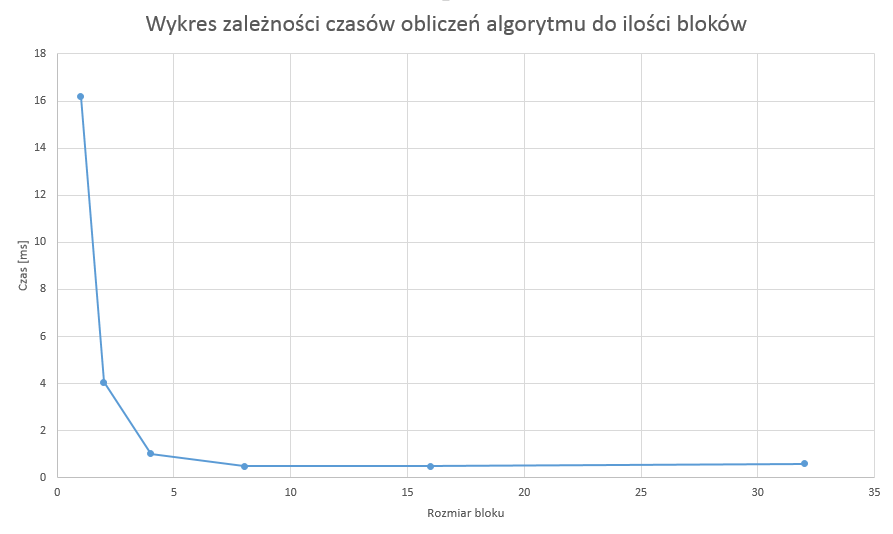
\includegraphics[width=0.5\textwidth]{Wykres1.PNG}
	\end{center}
	\vspace{-20pt}
	\caption{Wykres zależności czasów obliczeń do ilości bloków}
	\vspace{25pt}
\end{wrapfigure}
Na powyższym rysunku (Rysunek1) widzimy, że na przedziale 1 - 8 bloków czas obliczeńalgorytmu wraz ze wzrostem liczby bloków zmniejsza się parabolicznie aż do osiągnięcia stabilnego poziomu.
\begin{wrapfigure}{r}{0.5\textwidth}
	\vspace{0pt}
	\begin{center}
		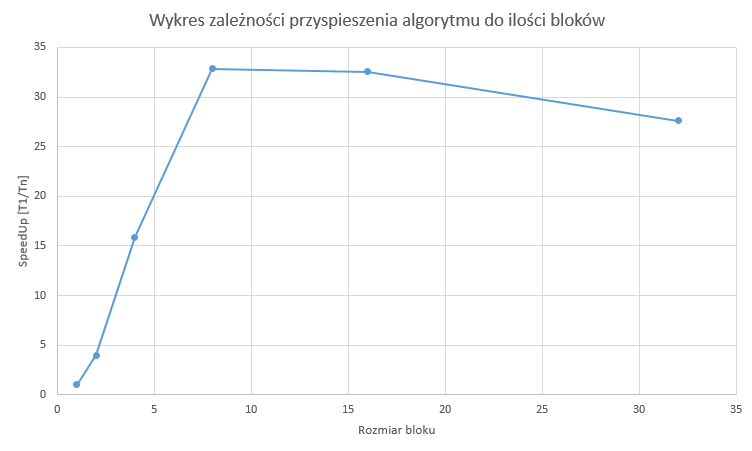
\includegraphics[width=0.5\textwidth]{Wykres2.PNG}
	\end{center}
	\vspace{-20pt}
	\caption{Wykres przyspieszenia}
	\vspace{35pt}
\end{wrapfigure}
Wykres zależności przyspieszenia algorytmu do ilości bloków obrazuje, że na przedziale 1 - 8 bloków CUDA ma bardzo duże przyspieszenie, następnie lekko się stabilizuje by na koniec nieco zwolnić.

\begin{wrapfigure}{r}{0.5\textwidth}
	\vspace{-40pt}
	\begin{center}
		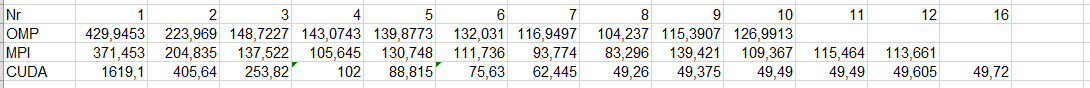
\includegraphics[width=0.5\textwidth]{tabelka_czasow.PNG}
	\end{center}
	\vspace{-20pt}
	\caption{Tabela czasów dla technologii OpenMP, MPI i CUDA}
	\vspace{35pt}
\end{wrapfigure}
Powyższa tabela przedstawia porównanie czasów przyspieszenia algorytmu do ilości bloków, dla trzech technologii: OpenMP, MPI oraz CUDA.
Zarówno z wyników w tabelce jak i na wykresie widzimy, że technologia CUDA ma bardzo duże przyspieszenie i osiąga najlepszy wynik w porównaniu 
do dwóch pozostałych technologii, a więc jest najbardziej wydajna dla tego typu zadania.

\begin{wrapfigure}{r}{0.5\textwidth}
	\vspace{-40pt}
	\begin{center}
		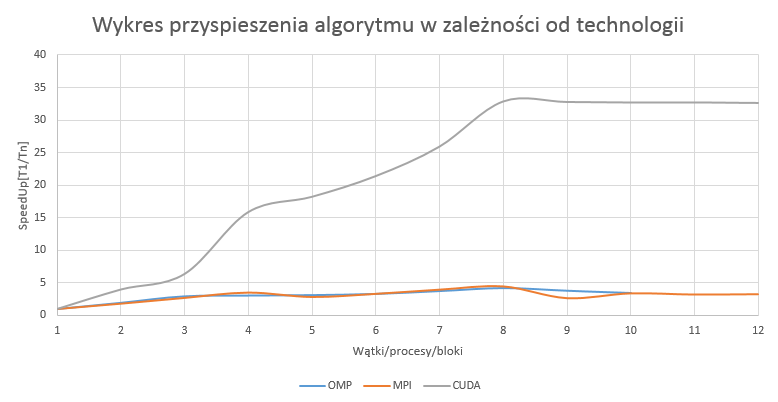
\includegraphics[width=0.5\textwidth]{zestawienie.PNG}
	\end{center}
	\vspace{-20pt}
	\caption{Wykres przyspieszenia}
	\vspace{35pt}
\end{wrapfigure}

\textbf{Podsumowanie:} CUDA (ang. Compute Unified Device Architecture) jest uniwersalną architekturą wielordzeniowych procesorów (głównie kart graficznych). Umożliwia wykorzystanie mocy obliczeniowej karty graficznej do rozwiązania problemów numerycznych w sposób wydajnieszy niż w tradycyjnych, sekwencyjnych procesorach ogólnego zastosowania.
Jednak zestawiając CUDA z dwoma pozostałymi technologiami MPI oraz OpenMP, czasowo wypada o wiele lepiej co świadczy o tym, że w przypadku rozmywania obrazka jest ona najbardziej wydajna. Algorytm Gaussa pozwolił nam w prosty i łatwy sposób dokonać rozmycia zadanej fotografii, a dzięki wcześniejszym laboratoriom z technologii CUDA, zastosowanie jej w niniejszym zadaniu nie stanowiło już dla nas większego problemu. 

\end{document}
